
%(BEGIN_QUESTION)
% Copyright 2007, Tony R. Kuphaldt, released under the Creative Commons Attribution License (v 1.0)
% This means you may do almost anything with this work of mine, so long as you give me proper credit

Graph the response of a proportional+integral controller to the following input conditions, assuming a proportional band of 100\% and an integral constant of 8 minutes per repeat.  The controller's action is {\it direct}, and the algorithm it follows is shown below the graph:

$$\includegraphics[width=15.5cm]{i01603x01.eps}$$

The time scale on the chart is minutes:seconds, and the PI algorithm is as follows:

$$m = K_p \left( e + {1 \over \tau_i} \int e \> dt \right) + b$$

\noindent
Where,

$m$ = Controller output (manipulated variable)

$K_p$ = Gain

$e$ = Error signal (PV$-$SP)

$\tau_i$ = Integral time constant

$b$ = Bias

\vskip 10pt

\underbar{file i01603}
%(END_QUESTION)





%(BEGIN_ANSWER)

$$\includegraphics[width=15.5cm]{i01603x02.eps}$$

%(END_ANSWER)





%(BEGIN_NOTES)

An integral constant of 8 minutes per repeat (0.125 repeats per minute) makes the output trace slope at a rather shallow (flat) rate.  It accumulates a 2.5\% output change in 1 minute.

%INDEX% Control, proportional + integral: graphing controller response

%(END_NOTES)


